\chapter{}

\section{Enunciado}

Paso de expresión regular a autómata finito y paso de autómata finito a expresión regular.

\section{Solución}

Para resolver este ejercicio elegimos la expresión regular para todas las cadenas que empiecen por \texttt{10} y justo después contengan una de las subcadenas \texttt{000} ó \texttt{111}:

\[10(000+111)\]

El siguiente autómata nos da la expresión regular \texttt{000}:

\begin{center}
\begin{tikzpicture}[-to, node distance=1.5cm]
	\node[state] (q4) []     {$q_{4}$};
	\node[state] (q5) [right of=q4] {$q_{5}$};
	\node[state] (q6) [right of=q5] {$q_{6}$};
	\node[state] (q7) [right of=q6] {$q_{7}$};
	\node[state] (q8) [right of=q7] {$q_{8}$};
	\node[state] (q9) [right of=q8] {$q_{9}$};

	\draw [arrows=->] (q4) -- (q5) node [midway,above] {$0$};
	\draw [arrows=->] (q5) -- (q6) node [midway,above] {$\epsilon$};
	\draw [arrows=->] (q6) -- (q7) node [midway,above] {$0$};
	\draw [arrows=->] (q7) -- (q8) node [midway,above] {$\epsilon$};
	\draw [arrows=->] (q8) -- (q9) node [midway,above] {$0$};
\end{tikzpicture}
\end{center}

También tenemos éste para \texttt{111}:

\begin{center}
\begin{tikzpicture}[-to, node distance=1.5cm]
	\node[state] (q10) []     {$q_{10}$};
	\node[state] (q11) [right of=q10] {$q_{11}$};
	\node[state] (q12) [right of=q11] {$q_{12}$};
	\node[state] (q13) [right of=q12] {$q_{13}$};
	\node[state] (q14) [right of=q13] {$q_{14}$};
	\node[state] (q15) [right of=q14] {$q_{15}$};

	\draw [arrows=->] (q10) -- (q11) node [midway,above] {$1$};
	\draw [arrows=->] (q11) -- (q12) node [midway,above] {$\epsilon$};
	\draw [arrows=->] (q12) -- (q13) node [midway,above] {$1$};
	\draw [arrows=->] (q13) -- (q14) node [midway,above] {$\epsilon$};
	\draw [arrows=->] (q14) -- (q15) node [midway,above] {$1$};
\end{tikzpicture}
\end{center}

Y, al princpio, el siguiente para \texttt{10}:

\begin{center}
\begin{tikzpicture}[-to, node distance=1.5cm]
	\node[state] (q0) []     {$q_{0}$};
	\node[state] (q1) [right of=q0] {$q_{1}$};
	\node[state] (q2) [right of=q1] {$q_{2}$};
	\node[state] (q3) [right of=q2] {$q_{3}$};

	\draw [arrows=->] (q0) -- (q1) node [midway,above] {$1$};
	\draw [arrows=->] (q1) -- (q2) node [midway,above] {$\epsilon$};
	\draw [arrows=->] (q2) -- (q3) node [midway,above] {$0$};
\end{tikzpicture}
\end{center}

Unimos los tres para formar el autómata final:

\begin{center}
\begin{tikzpicture}[-to, node distance=1.5cm]
	\node[state,initial] (q0) [] {$q_{0}$};
	\node[state]         (q1) [right of=q0] {$q_{1}$};
	\node[state]         (q2) [right of=q1] {$q_{2}$};
	\node[state]         (q3) [right of=q2] {$q_{3}$};

	\draw [arrows=->] (q0) -- (q1) node [midway,above] {$1$};
	\draw [arrows=->] (q1) -- (q2) node [midway,above] {$\epsilon$};
	\draw [arrows=->] (q2) -- (q3) node [midway,above] {$0$};

	\node[state] (q4) [above right of=q3] {$q_{4}$};
	\node[state] (q5) [right of=q4]       {$q_{5}$};
	\node[state] (q6) [right of=q5]       {$q_{6}$};
	\node[state] (q7) [right of=q6]       {$q_{7}$};
	\node[state] (q8) [right of=q7]       {$q_{8}$};
	\node[state] (q9) [right of=q8]       {$q_{9}$};

	\draw [arrows=->] (q3) -- (q4) node [midway,above] {$\epsilon$};
	\draw [arrows=->] (q4) -- (q5) node [midway,above] {$0$};
	\draw [arrows=->] (q5) -- (q6) node [midway,above] {$\epsilon$};
	\draw [arrows=->] (q6) -- (q7) node [midway,above] {$0$};
	\draw [arrows=->] (q7) -- (q8) node [midway,above] {$\epsilon$};
	\draw [arrows=->] (q8) -- (q9) node [midway,above] {$0$};

	\node[state] (q10) [below right of=q3] {$q_{10}$};
	\node[state] (q11) [right of=q10]      {$q_{11}$};
	\node[state] (q12) [right of=q11]      {$q_{12}$};
	\node[state] (q13) [right of=q12]      {$q_{13}$};
	\node[state] (q14) [right of=q13]      {$q_{14}$};
	\node[state] (q15) [right of=q14]      {$q_{15}$};

	\draw [arrows=->] (q3)  -- (q10) node [midway,below] {$\epsilon$};
	\draw [arrows=->] (q10) -- (q11) node [midway,above] {$1$};
	\draw [arrows=->] (q11) -- (q12) node [midway,above] {$\epsilon$};
	\draw [arrows=->] (q12) -- (q13) node [midway,above] {$1$};
	\draw [arrows=->] (q13) -- (q14) node [midway,above] {$\epsilon$};
	\draw [arrows=->] (q14) -- (q15) node [midway,above] {$1$};

	\node[state,accepting] (q16) [above  right of=q15] {$q_{16}$};

	\draw [arrows=->] (q9)  -- (q16) node [midway,above] {$\epsilon$};
	\draw [arrows=->] (q15) -- (q16) node [midway,below] {$\epsilon$};
\end{tikzpicture}
\end{center}

Para la operación inversa vamos a trabajar con el siguiente autómata:

\begin{center}
\begin{tikzpicture}[-to, node distance=1.5cm]
	\node[state,initial] (q0) [] {$q_{0}$};
	\node[state]         (q1) [right of=q0] {$q_{1}$};

	\draw [arrows=->] (q0) -- (q1) node [midway,above] {$1$};

	\node[state] (q2) [above right of=q1] {$q_{2}$};
	\node[state] (q3) [right of=q2]       {$q_{3}$};

	\draw [arrows=->] (q1) -- (q2) node [midway,above] {$\epsilon$};
	\draw [arrows=->] (q2) -- (q3) node [midway,above] {$0$};

	\node[state] (q4) [below right of=q1] {$q_{4}$};
	\node[state] (q5) [right of=q4]       {$q_{5}$};

	\draw [arrows=->] (q1) -- (q4) node [midway,below] {$\epsilon$};
	\draw [arrows=->] (q4) -- (q5) node [midway,above] {$1$};

	\node[state]           (q6) [below right of=q3] {$q_{6}$};
	\node[state,accepting] (q7) [right of=q6]       {$q_{7}$};

	\draw [arrows=->] (q3) -- (q6) node [midway,above] {$\epsilon$};
	\draw [arrows=->] (q5) -- (q6) node [midway,below] {$\epsilon$};
	\draw [arrows=->] (q6) -- (q7) node [midway,above] {$0$};
\end{tikzpicture}
\end{center}

\pagebreak

Para este ejercicio utilizamos jFlap, que nos permite descubrir la expresión regular resultante de un autómata finito.
Utilizando la opción \textit{Convert FA to RE}, nos da la siguiente expresión:

\[100+110\]

\begin{figure}[h!]
\begin{center}
	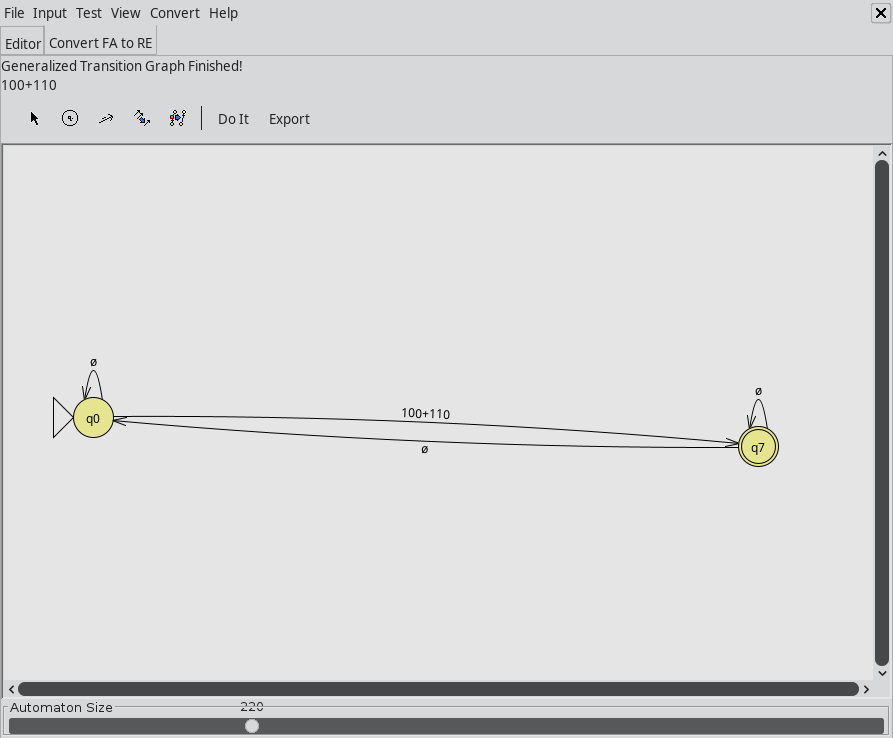
\includegraphics[scale=0.70]{Problemas/jFlap - Regex a AF}
\caption{Resultado de conversión del autómata en jFlap.}
\end{center}
\end{figure}
